% Options for packages loaded elsewhere
\PassOptionsToPackage{unicode}{hyperref}
\PassOptionsToPackage{hyphens}{url}
\PassOptionsToPackage{dvipsnames,svgnames,x11names}{xcolor}
%
\documentclass[
]{article}

\usepackage{amsmath,amssymb}
\usepackage{lmodern}
\usepackage{iftex}
\ifPDFTeX
  \usepackage[T1]{fontenc}
  \usepackage[utf8]{inputenc}
  \usepackage{textcomp} % provide euro and other symbols
\else % if luatex or xetex
  \usepackage{unicode-math}
  \defaultfontfeatures{Scale=MatchLowercase}
  \defaultfontfeatures[\rmfamily]{Ligatures=TeX,Scale=1}
\fi
% Use upquote if available, for straight quotes in verbatim environments
\IfFileExists{upquote.sty}{\usepackage{upquote}}{}
\IfFileExists{microtype.sty}{% use microtype if available
  \usepackage[]{microtype}
  \UseMicrotypeSet[protrusion]{basicmath} % disable protrusion for tt fonts
}{}
\usepackage{xcolor}
\usepackage[top=20mm,left=18mm,right=18mm,heightrounded]{geometry}
\setlength{\emergencystretch}{3em} % prevent overfull lines
\setcounter{secnumdepth}{5}
% Make \paragraph and \subparagraph free-standing
\ifx\paragraph\undefined\else
  \let\oldparagraph\paragraph
  \renewcommand{\paragraph}[1]{\oldparagraph{#1}\mbox{}}
\fi
\ifx\subparagraph\undefined\else
  \let\oldsubparagraph\subparagraph
  \renewcommand{\subparagraph}[1]{\oldsubparagraph{#1}\mbox{}}
\fi


\providecommand{\tightlist}{%
  \setlength{\itemsep}{0pt}\setlength{\parskip}{0pt}}\usepackage{longtable,booktabs,array}
\usepackage{calc} % for calculating minipage widths
% Correct order of tables after \paragraph or \subparagraph
\usepackage{etoolbox}
\makeatletter
\patchcmd\longtable{\par}{\if@noskipsec\mbox{}\fi\par}{}{}
\makeatother
% Allow footnotes in longtable head/foot
\IfFileExists{footnotehyper.sty}{\usepackage{footnotehyper}}{\usepackage{footnote}}
\makesavenoteenv{longtable}
\usepackage{graphicx}
\makeatletter
\def\maxwidth{\ifdim\Gin@nat@width>\linewidth\linewidth\else\Gin@nat@width\fi}
\def\maxheight{\ifdim\Gin@nat@height>\textheight\textheight\else\Gin@nat@height\fi}
\makeatother
% Scale images if necessary, so that they will not overflow the page
% margins by default, and it is still possible to overwrite the defaults
% using explicit options in \includegraphics[width, height, ...]{}
\setkeys{Gin}{width=\maxwidth,height=\maxheight,keepaspectratio}
% Set default figure placement to htbp
\makeatletter
\def\fps@figure{htbp}
\makeatother
\newlength{\cslhangindent}
\setlength{\cslhangindent}{1.5em}
\newlength{\csllabelwidth}
\setlength{\csllabelwidth}{3em}
\newlength{\cslentryspacingunit} % times entry-spacing
\setlength{\cslentryspacingunit}{\parskip}
\newenvironment{CSLReferences}[2] % #1 hanging-ident, #2 entry spacing
 {% don't indent paragraphs
  \setlength{\parindent}{0pt}
  % turn on hanging indent if param 1 is 1
  \ifodd #1
  \let\oldpar\par
  \def\par{\hangindent=\cslhangindent\oldpar}
  \fi
  % set entry spacing
  \setlength{\parskip}{#2\cslentryspacingunit}
 }%
 {}
\usepackage{calc}
\newcommand{\CSLBlock}[1]{#1\hfill\break}
\newcommand{\CSLLeftMargin}[1]{\parbox[t]{\csllabelwidth}{#1}}
\newcommand{\CSLRightInline}[1]{\parbox[t]{\linewidth - \csllabelwidth}{#1}\break}
\newcommand{\CSLIndent}[1]{\hspace{\cslhangindent}#1}

\usepackage{float}
\makeatletter
\makeatother
\makeatletter
\makeatother
\makeatletter
\@ifpackageloaded{caption}{}{\usepackage{caption}}
\AtBeginDocument{%
\ifdefined\contentsname
  \renewcommand*\contentsname{Índice}
\else
  \newcommand\contentsname{Índice}
\fi
\ifdefined\listfigurename
  \renewcommand*\listfigurename{Lista de Figuras}
\else
  \newcommand\listfigurename{Lista de Figuras}
\fi
\ifdefined\listtablename
  \renewcommand*\listtablename{Lista de Tabelas}
\else
  \newcommand\listtablename{Lista de Tabelas}
\fi
\ifdefined\figurename
  \renewcommand*\figurename{Figura}
\else
  \newcommand\figurename{Figura}
\fi
\ifdefined\tablename
  \renewcommand*\tablename{Tabela}
\else
  \newcommand\tablename{Tabela}
\fi
}
\@ifpackageloaded{float}{}{\usepackage{float}}
\floatstyle{ruled}
\@ifundefined{c@chapter}{\newfloat{codelisting}{h}{lop}}{\newfloat{codelisting}{h}{lop}[chapter]}
\floatname{codelisting}{Listagem}
\newcommand*\listoflistings{\listof{codelisting}{Lista de Listagens}}
\makeatother
\makeatletter
\@ifpackageloaded{caption}{}{\usepackage{caption}}
\@ifpackageloaded{subcaption}{}{\usepackage{subcaption}}
\makeatother
\makeatletter
\@ifpackageloaded{tcolorbox}{}{\usepackage[many]{tcolorbox}}
\makeatother
\makeatletter
\@ifundefined{shadecolor}{\definecolor{shadecolor}{rgb}{.97, .97, .97}}
\makeatother
\makeatletter
\makeatother
\ifLuaTeX
\usepackage[bidi=basic]{babel}
\else
\usepackage[bidi=default]{babel}
\fi
\babelprovide[main,import]{portuguese}
% get rid of language-specific shorthands (see #6817):
\let\LanguageShortHands\languageshorthands
\def\languageshorthands#1{}
\ifLuaTeX
  \usepackage{selnolig}  % disable illegal ligatures
\fi
\IfFileExists{bookmark.sty}{\usepackage{bookmark}}{\usepackage{hyperref}}
\IfFileExists{xurl.sty}{\usepackage{xurl}}{} % add URL line breaks if available
\urlstyle{same} % disable monospaced font for URLs
\hypersetup{
  pdftitle={Distribuição Kumaraswamy},
  pdfauthor={Alisson Rosa,   Digite seu nome aqui!},
  pdflang={pt},
  colorlinks=true,
  linkcolor={blue},
  filecolor={Maroon},
  citecolor={Blue},
  urlcolor={Blue},
  pdfcreator={LaTeX via pandoc}}

\title{Distribuição Kumaraswamy}
\usepackage{etoolbox}
\makeatletter
\providecommand{\subtitle}[1]{% add subtitle to \maketitle
  \apptocmd{\@title}{\par {\large #1 \par}}{}{}
}
\makeatother
\subtitle{E suas Aplicações}
\author{Alisson Rosa, Digite seu nome aqui!}
\date{}

\begin{document}
\maketitle
\begin{abstract}
Muitas vezes estamos interessados em modelar variáveis que estão
definidas entre zero e um, como sabemos aonde nossa variável esta
definida mas não sabemos qual dos valores será observado, temos portanto
uma incerteza probabilística, que pode e deve ser modelada por medidas
de probabilidade. Aqui portanto, introduziremos a distribuição
Kumaraswamy, que é uma das muitas possibilidades para modelagem desse
tipo de variável, encontraremos estimativas para os parâmetros da
distribuição usando estimadores de máxima verossimilhança blah blah.
\end{abstract}
\ifdefined\Shaded\renewenvironment{Shaded}{\begin{tcolorbox}[boxrule=0pt, enhanced, borderline west={3pt}{0pt}{shadecolor}, frame hidden, sharp corners, breakable, interior hidden]}{\end{tcolorbox}}\fi

\section{\centering Introdução}

Atualmente muitos fenômenos podem ser descritos como variáveis
aleatórias (va) definidas no intervalo unitário (0,1) \footnote{Onde
  parenteses indica limites do intervalo abertos.}, assim é natural que
pesquisadores desenvolvam distribuições de probabilidade que abarcam
esse tipo de va. Uma dessas distribuições é a Kumaraswamy, que foi
introduzida em Kumaraswamy (1980) como uma alternativa ao modelo beta
para aplicações na ́area de hidrologia. Em virtude deste fato, grande
parte dos trabalhos empíricos desta distribuição concentra-se nessa área
Nadarajah (2008). O presente trabalho visa contribuir na expansão e
utilização da Kumaraswamy, empregando modelos incondicionais para a taxa
de desfloresmento em diversos munícipios da Amazônia legal,
disponilizados
(http://www.dpi.inpe.br/prodesdigital/prodesmunicipal.php){[}aqui{]}
pelo projeto PRODES do INPE. Assim é possível mensurar a qualidade da
Kumaraswamy para modelagem dos dados propostos, para isso estamos
utilizando 6 métricas frequentistas estabelecidas: AIC, BIC, CAIC,
Kolmogorov-Smirnov, Cramer-Von Mises e Anderson-Darling, em contraste
com a Distribuição Normal e a Distribuição Beta.

\section{\centering A distribuição Kumaraswamy}

Vamos nessa seção introduzir quantidades básicas da distribuição
Kumaraswamy, sendo elas sua função densidade de probabilidade (pdf),
função de distribuição acumulada (cdf), função quantilica (qf), função
de verossimilhança (ll) e esperança (\textbf{E})

\subsection{Quantidade Básicas}

Seja X uma variável aleatória que segue uma distribuição Kumaraswamy,
então sua cdf é dada por:

\begin{align}
F(x;\alpha, \beta) = 1 - (1 - x^\alpha)^\beta,  \quad 0 < x< 1
\end{align}

Onde \(\alpha, \beta > 0\). Sua pdf então fica definida como:

\begin{align}
f(x;\alpha, \beta) = \dfrac{dF}{dx} =\alpha\beta x^{\alpha - 1}(1 - x^\alpha)^{\beta  - 1}, \quad 0 < x< 1
\end{align}

Sua qf, que é a função inversa da cdf, fica definida como:

\begin{align}
Q(u;\alpha, \beta) = \bigg(1 - (1 - u)^{1/\beta}\bigg)^{\dfrac{1}{\alpha}}, \quad 0<u<1
\end{align}

É FÁCIL ver que que a esperança da distribuição Kumaraswamy é dada por

\begin{align}
\text{E}(X) = \dfrac{\beta\Gamma\bigg(1 + \dfrac{1}{\alpha}\bigg)\Gamma(\beta)}{\Gamma\bigg(1 + \dfrac{1}{\alpha} + \beta\bigg)}
\end{align}

A função de verossimilhança é dada por:

\begin{align}
L(\alpha, \beta; x) = \prod_{i=1}^{n}f(x;\alpha, \beta) = \alpha^n \beta^n \prod_{i=1}^{n}x_i^{\alpha - 1}\prod_{i=1}^{n}(1-x_i^{\alpha})^{\beta-1}
\end{align}

\begin{figure}

{\centering 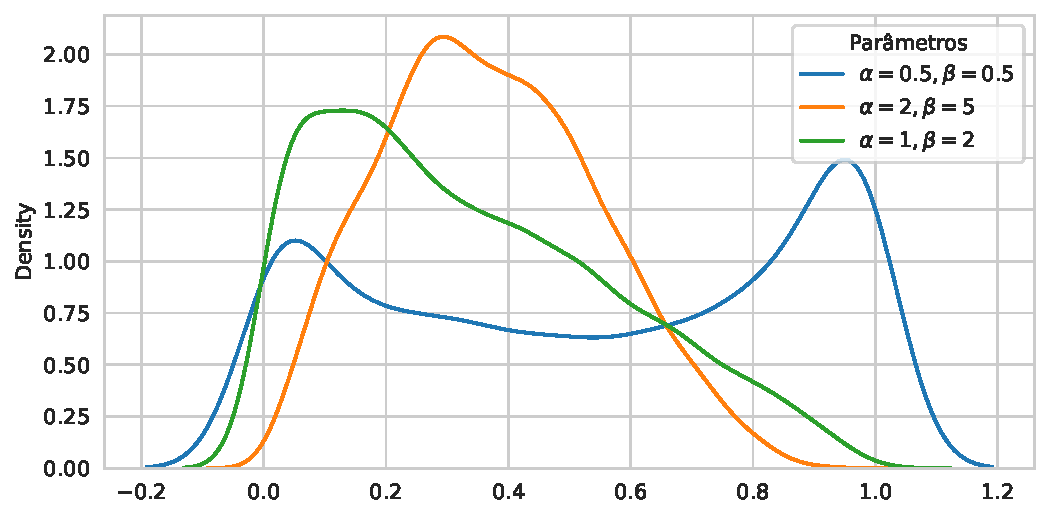
\includegraphics{report_files/figure-pdf/fig-plt-output-1.pdf}

}

\caption{\label{fig-plt}Função densidade da Kumaraswamy para alguns
valores de parâmetros}

\end{figure}

\subsection{Justificativa}

O artigo de Kumaraswamy (1980) propõe e demonstra aplicações da
distribuição Kumaraswamy para variáveis aleatórias e processos
aleatórios derivados de processos hidrológicos. O artigo foi publicado
na \emph{Journal of Hydrology}, assim é perceptível que a distribuição
foi concebida para se adequar a dados hidrológicos. Temos como casos de
suas utilizações em precipitação diária, fluxo diário, reservatórios de
água e análise das ondas do oceano, entre outras.

Para Nadarajah (2008) a utilização da Kumaraswamy para o campo da
hidrologia, é consolidada. Sendo perceptível pelas inúmeras aplicações
em diversos artigos como: Sundar e Subbiah (1989), Fletcher e
Ponnambalam (2008) e Koutsoyiannis e Xanthopoulos (1989), além de se
sobressair em relação a distribuição beta, a distribuição padrão para
dados no (0,1), de acordo com Koutsoyiannis e Xanthopoulos (1989). Em
Dey, Mazucheli, e Nadarajah (2018) a Kumaraswamy é utilizada para a
quantidade de deslocamento de líquido metálico em duas máquinas
diferentes, sendo superior as Distribuições Gumbel e Fréchet.

É notório também a dissiminação recente do estudo da Kumaraswamy, em
expansão para distribuições mais complexas, como em Lemonte,
Barreto-Souza, e Cordeiro (2013), Mazucheli et al. (2020), Cribari-Neto
e Santos (2019) e Sagrillo, Guerra, e Bayer (2021) ou em suas aplicações
em regressão e séries temporais, visto em Pumi, Rauber, e Bayer (2020),
Mitnik e Baek (2013), Fábio M. Bayer, Cribari-Neto, e Santos (2021) e
Fábio Mariano Bayer, Bayer, e Pumi (2017).

Assim é factível a falta de ajustes da Distribuição Kumaraswamy em
outras áreas de estudo, visto que a Kumaraswamy tem dissiminação
acadêmica exponencial recentemente, com admiráveis contribuições da
UFSM, em artigos supracitados. Decidimos contribuir para um maior estudo
da distribuição em outra área ambiental, o desmatamento, pensando
especificamente na Amazônia brasileira.

O estudo e modelos com bons ajustes de desmatamento e desflorestamento,
impactam a vida no mundo todo, tanto humana quanto não humana. Bons
modelos conseguem prever e informar quais variáveis mais impactam nos
desmatamento, possibilitando verificar sua evolução conforme o tempo.
Sendo útil para construção de políticas públicas, visando tomadas de
decisão mais eficientes.

O desflorestamento é questão com importância ambiental, social,
econômica e até política, pois a floresta amazônica tem seu papel no
armazenamento de carbono, evitando o aquecimento global, na reciclagem
de água e na manutenção da biodiversidade. Além de fornecerem uma grande
variedade de produtos materiais e de sustento para as populações locais.
Mesmo com áreas com grandes partes preservadas, há impacto na
biodiversidade, pois a distribuição das espécies não é uniforme. Muitas
espécies têm áreas de ocorrência restritas a partes que já foram
reduzida a pequenos fragmentos.

\section{\centering Análise Inicial}

blah blah

\subsection{Apresentação dos dados}

\begin{figure}

{\centering 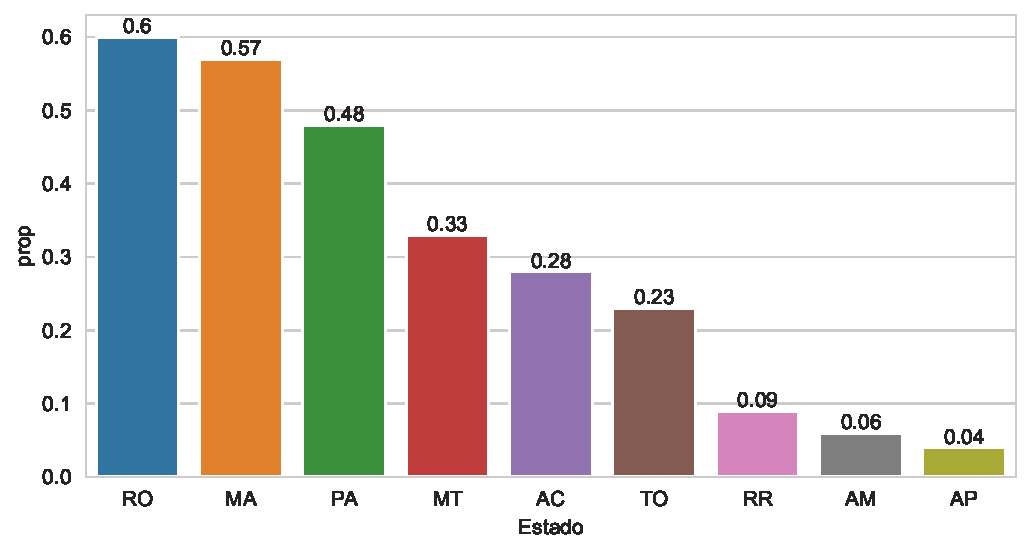
\includegraphics{report_files/figure-pdf/fig-states-output-1.pdf}

}

\caption{\label{fig-states}Proporção média dos Estados}

\end{figure}

\subsection{Medidas Básicas}

\section{\centering Ajuste do Modelo}

Para a verificação da adequação da distribuição Kumaraswamy para
modelagem de dados de desmatamento iremos realizar a comparação com duas
distribuições amplamente utilizadas: Distribuição Normal e a
Distribuição beta, a distribuição mais utilizada para variáveis
aleatórias com suporte no (0,1).

A comparação foi construída utilizando 6 métricas: AIC, BIC, CAIC,
Kolmogorov-Smirnov, Cramer-Von Mises e Anderson-Darling, que se baseiam
principalmente na verossimilhança. A verossimilhança a considera os
parâmetros variáveis, assim a função de verossimilhança indica os
parâmetros mais plausíveis de terem gerado a amostra. Logo, podemos
verificar entre todas as distribuições quais possuem as maiores
verossimilhanças, tendo assim os parâmetros mais plausíveis para a
geração da amostra. No entanto, nota-se que todos os critérios contam
outros elementos para a sua construção.

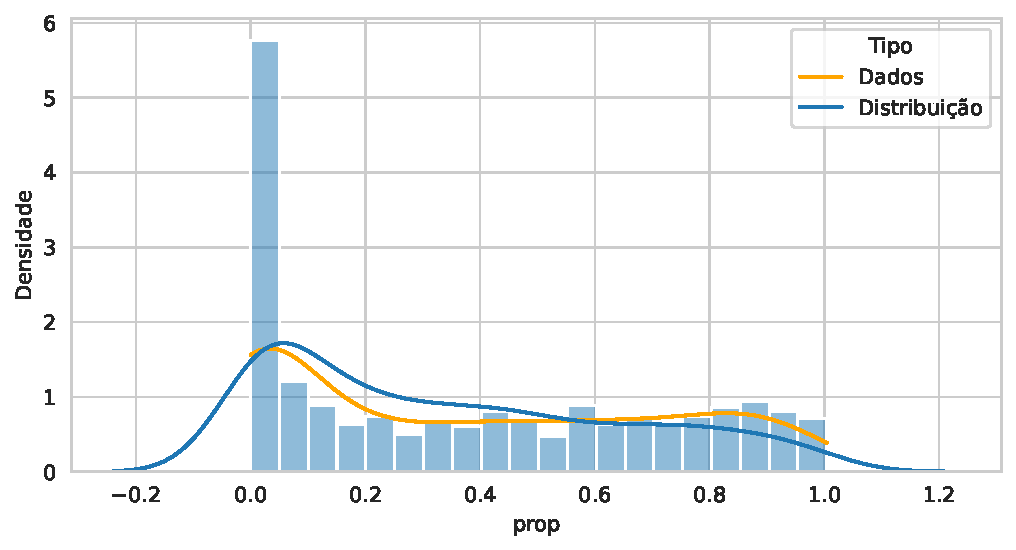
\includegraphics{report_files/figure-pdf/cell-6-output-1.pdf}

\begin{tabular}{lrrrl}
\toprule
{} &  Kumaraswamy &        Beta &         Normal & Vencedor \\
\midrule
0 &  -440.933936 & -443.086140 & -154637.091792 &   Normal \\
1 &  -440.918084 & -433.819504 & -154627.825155 &   Normal \\
2 &  -431.667299 & -443.070288 & -154637.075940 &   Normal \\
3 &    18.106283 &    9.736648 &     767.892814 &   Normal \\
4 &     9.691977 &    1.251566 &      64.378061 &   Normal \\
5 &     0.088746 &    0.089166 &       0.537076 &   Normal \\
\bottomrule
\end{tabular}

\section{\centering Conclusão}

\section{\centering Referências}

\hypertarget{refs}{}
\begin{CSLReferences}{1}{0}
\leavevmode\vadjust pre{\hypertarget{ref-bayer2017kumaraswamy}{}}%
Bayer, Fábio Mariano, Débora Missio Bayer, e Guilherme Pumi. 2017.
{"Kumaraswamy autoregressive moving average models for double bounded
environmental data"}. \emph{Journal of Hydrology} 555: 385--96.

\leavevmode\vadjust pre{\hypertarget{ref-bayer2021inflated}{}}%
Bayer, Fábio M, Francisco Cribari-Neto, e Jéssica Santos. 2021.
{"Inflated Kumaraswamy regressions with application to water supply and
sanitation in Brazil"}. \emph{Statistica Neerlandica} 75 (4): 453--81.

\leavevmode\vadjust pre{\hypertarget{ref-cribari2019inflated}{}}%
Cribari-Neto, Francisco, e Jessica Santos. 2019. {"Inflated Kumaraswamy
distributions"}. \emph{Anais da Academia Brasileira de Ci{ê}ncias} 91.

\leavevmode\vadjust pre{\hypertarget{ref-dey2018kumaraswamy}{}}%
Dey, Sanku, Josmar Mazucheli, e Saralees Nadarajah. 2018. {"Kumaraswamy
distribution: different methods of estimation"}. \emph{Computational and
Applied Mathematics} 37 (2): 2094--2111.

\leavevmode\vadjust pre{\hypertarget{ref-fletcher}{}}%
Fletcher, SG, e K Ponnambalam. 2008. {"Stochastic control of reservoir
systems using indicator functions: new enhancements"}. \emph{Water
Resources Research} 44 (12).

\leavevmode\vadjust pre{\hypertarget{ref-ganji2006grain}{}}%
Ganji, A, K Ponnambalam, D Khalili, e M Karamouz. 2006. {"Grain yield
reliability analysis with crop water demand uncertainty"}.
\emph{Stochastic Environmental Research and Risk Assessment} 20 (4):
259--77.

\leavevmode\vadjust pre{\hypertarget{ref-koutsoyiannis}{}}%
Koutsoyiannis, Demetris, e Themistocle Xanthopoulos. 1989. {"On the
parametric approach to unit hydrograph identification"}. \emph{Water
resources management} 3 (2): 107--28.

\leavevmode\vadjust pre{\hypertarget{ref-kuma}{}}%
Kumaraswamy, Ponnambalam. 1980. {"A generalized probability density
function for double-bounded random processes"}. \emph{Journal of
hydrology} 46 (1-2): 79--88.

\leavevmode\vadjust pre{\hypertarget{ref-lemonte2013exponentiated}{}}%
Lemonte, Artur J, Wagner Barreto-Souza, e Gauss M Cordeiro. 2013. {"The
exponentiated Kumaraswamy distribution and its log-transform"}.
\emph{Brazilian Journal of Probability and Statistics} 27 (1): 31--53.

\leavevmode\vadjust pre{\hypertarget{ref-mazucheli2020unit}{}}%
Mazucheli, J, AFB Menezes, LB Fernandes, RP De Oliveira, e ME Ghitany.
2020. {"The unit-Weibull distribution as an alternative to the
Kumaraswamy distribution for the modeling of quantiles conditional on
covariates"}. \emph{Journal of Applied Statistics} 47 (6): 954--74.

\leavevmode\vadjust pre{\hypertarget{ref-mitnik2013new}{}}%
Mitnik, Pablo A. 2013. {"New properties of the Kumaraswamy
distribution"}. \emph{Communications in Statistics-Theory and Methods}
42 (5): 741--55.

\leavevmode\vadjust pre{\hypertarget{ref-mitnik2013kumaraswamy}{}}%
Mitnik, Pablo A, e Sunyoung Baek. 2013. {"The Kumaraswamy distribution:
median-dispersion re-parameterizations for regression modeling and
simulation-based estimation"}. \emph{Statistical Papers} 54 (1):
177--92.

\leavevmode\vadjust pre{\hypertarget{ref-nadarajah2008distribution}{}}%
Nadarajah, Saralees. 2008. {"On the distribution of Kumaraswamy"}.
\emph{Journal of Hydrology} 348 (3): 568--69.

\leavevmode\vadjust pre{\hypertarget{ref-pumi2020kumaraswamy}{}}%
Pumi, Guilherme, Cristine Rauber, e Fábio M Bayer. 2020. {"Kumaraswamy
regression model with Aranda-Ordaz link function"}. \emph{Test} 29 (4):
1051--71.

\leavevmode\vadjust pre{\hypertarget{ref-r}{}}%
R Core Team. 2022. \emph{R: A Language and Environment for Statistical
Computing}. Vienna, Austria: R Foundation for Statistical Computing.
\url{https://www.R-project.org/}.

\leavevmode\vadjust pre{\hypertarget{ref-sagrillo2021modified}{}}%
Sagrillo, Murilo, Renata Rojas Guerra, e Fábio M Bayer. 2021. {"Modified
Kumaraswamy distributions for double bounded hydro-environmental data"}.
\emph{Journal of Hydrology} 603: 127021.

\leavevmode\vadjust pre{\hypertarget{ref-sundar}{}}%
Sundar, V, e K Subbiah. 1989. {"Application of double bounded
probability density function for analysis of ocean waves"}. \emph{Ocean
engineering} 16 (2): 193--200.

\end{CSLReferences}



\end{document}
